
\section{\sysname 系统概览}
\label{sec:system-overview}

为打破 prefill 侧存储 I/O 瓶颈，我们提出一种\textbf{双路径加载}架构，从根本上重新思考 PD 解耦推理中 KV-Cache 的取回方式。基于该架构，我们设计并实现了 \sysname。
\sysname 采用 \autoref{sec:background} 中介绍的两项被广泛采用的技术：
(1) \textbf{PD 解耦}~\cite{OSDI24:DistServe,ISCA24:Splitwise}，将 prompt 处理与 decode 处理分离以提升效率。
(2) \textbf{逐层 prefill}，它避免了 LayerKV~\cite{LayerKV} 和 PrefillOnly~\cite{SOSP25:PrefillOnly} 所指出的 prefill engine 上 HBM 瓶颈，并提高 GPU 利用率。

我们的系统由以下组件组成：
\begin{itemize}[leftmargin=*]
    \item \textbf{推理 Engine。} 每个 engine 管理一块 GPU。
    Engine 分为用于 prefill 的 prefill engine（PE）和用于 decode 的 decode engine（DE）。
    \item \textbf{流量管理器（\autoref{sec:traffic-manager}）。} 每个 engine 都包含一个流量管理器，用于执行：（1）Host-Device 内存拷贝（H2D 与 D2H），（2）PE 与 DE 之间的 KV-Cache 传输，以及（3）通过存储 NIC 从存储读取/向存储写入 KV-Cache。我们采用以 CNIC 为中心的流量管理方式，详见 \autoref{sec:traffic-manager}，以防 KV-Cache 流量影响模型推理通信。
    \item \textbf{请求 Scheduler（\autoref{sec:scheduling}）。} 中央 scheduler 接收客户端请求并将其分发到各个 engine。它还负责在两条路径之间动态分配数据流量（\autoref{fig:dual-path-loading}）。
\end{itemize}

\begin{figure*}[t!]
  \centering
   \begin{subfigure}[b]{0.45\textwidth}
     \centering
      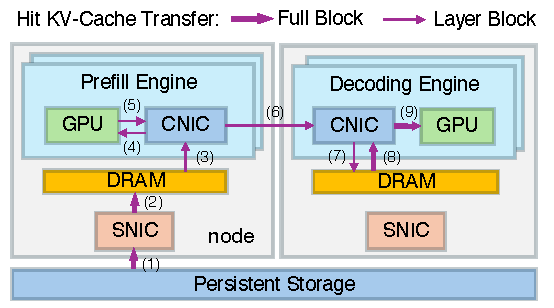
\includegraphics[width=\textwidth]{figures/dataflow_peread.pdf}
      \caption{\normalfont PE 读取路径}
      \label{fig:pe_flow}
    \end{subfigure}
    \hspace{6mm}
    \begin{subfigure}[b]{0.45\textwidth}
        \centering
      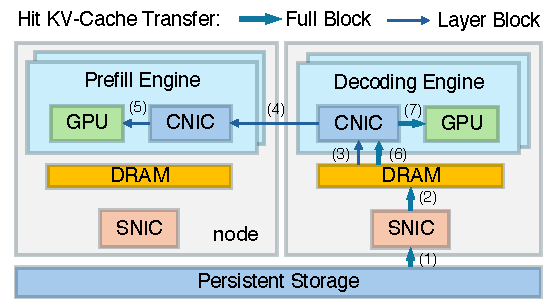
\includegraphics[width=\textwidth]{figures/dataflow_ceread.pdf}
      \caption{\normalfont DE 读取路径}
      \label{fig:de_flow}  
    \end{subfigure}
    \caption{\normalfont 双路径加载示意图。Scheduler 在两条路径之间动态分配数据流量。}
    \label{fig:dual-path-loading}
\end{figure*}


\subsection{双路径加载}
\label{sec:dual-path-loading}

除传统的\emph{storage-to-prefill} 路径之外，\sysname 引入了一条新的\emph{storage-to-decode} 路径，使 KV-Cache 可以先被加载到 decode engine，再通过计算网络上的高带宽 RDMA 传输到 prefill engine。
通过在两条路径之间动态分配负载，系统能够聚合所有 engine 的存储 NIC 带宽，包括原本空闲的 decode 侧 NIC，并消除限制现有系统的不对称带宽饱和问题。这种方式将存储 I/O 从单一瓶颈资源转化为一个全局池化且可调度的容量。% The following subsections detail the data-flow design and prove its feasibility under typical deployment ratios.
双路径的具体数据流如下。

为实现双路径加载，\sysname 在每个 PE 和 DE 上分配少量 DRAM 作为 buffer，分别称为 \emph{PE buffer} 和 \emph{DE Buffer}。
% In \autoref{fig:pe_flow} and \autoref{fig:de_flow}, we ignore all newly computed KV-Cache, since its volume is bounded by the GPU's compute capacity and is therefore relatively small.

\parabf{Prefill PE 读取路径。}
首先，命中 token 的 KV-Cache 从持久化存储读入 PE buffer（如 \autoref{fig:pe_flow} 中标签 1 和 2 所示）。
在计算某个 attention 层之前，该层的 KV-Cache 被传输到 PE HBM（3 和 4），用于计算 cache-miss prompt token 的 KV-Cache。
随后，命中和未命中 token 的全部 KV-Cache 都被传输到 DE buffer，形成完整的 prompt KV-Cache（5-7）。该过程（3-7）重复 $n_{layer}$ 次。
在 prefill forward 过程中，传输会与计算重叠。

\parabf{Prefill DE 读取路径。} 命中 token 的 KV-Cache 首先被读入 DE buffer（如 \autoref{fig:de_flow} 中标签 1 和 2 所示）。
在 PE prefill 期间，对应层的 KV-Cache 从 DE buffer 读取，同样与计算重叠（3-5）。该过程重复 $n_{layer}$ 次。
当一层计算完成后，只有 miss token 的 KV-Cache 会被传输到 DE buffer，并与已有的 hit token KV-Cache 合并。

\parabf{Decode 阶段。} 当 DE buffer 中收到完整的 prompt KV-Cache 后（包括通过 PE 读取路径加载的 KV-Cache，以及新追加 token 的 KV-Cache），decode 阶段开始。
DE 首先分配 HBM 并执行 host-to-device（H2D）传输（\autoref{fig:pe_flow} 中标签 8 和 9；\autoref{fig:de_flow} 中标签 6 和 7），随后在开始 decode 前释放 CPU 内存。
DE buffer 的设计会对 DRAM 和 CNIC 施加带宽压力（额外一次 H2D），这本可通过 GPU Direct RDMA 直接绕过 buffer 来避免。
然而，由于该场景下 generation length 通常较短，time-to-first-token（TTFT）在端到端请求时间中占据不可忽视的比例。
引入 DE buffer 有助于降低 GPU 内存使用。
在 decode 过程中，一旦累积出一个完整 token block（例如 64 个 token），系统会立即将其持久化到磁盘。

\parabf{不同 Block 布局。}
我们采用两种不同 block 布局：\emph{Full Block} 和 \emph{Layer Block}，分别包含所有层和单层。
详细布局见 \autoref{subsec:block-layout}。
对于所有与存储的交互，我们使用 Full Block。
在 PE 读取场景中，将 KV-Cache 加载到 PE HBM 以及传输到 DE Buffer 都以逐层流式方式进行，二者均使用 Layer Block。
类似地，对于 DE 读取路径，从 DE Buffer 到 PE HBM 的传输也使用 Layer Block。




\subsection{无瓶颈分析}
\label{subsec:bottle-free-analysis}
我们证明，在大多数合理 P/D 比例下，系统可以充分打满所有存储 NIC，而不会引入 compute-NIC 或 DRAM 瓶颈。
我们假设 PCIe 拓扑配置合理（每对 GPU--NIC 位于同一 PCIe switch 下）、任务调度负载均衡、计算网络无拥塞，并且存储读取带宽被充分利用。

\parabf{符号。} 令 $P$ 和 $D$ 分别表示 prefill 节点和 decode 节点数量。每个节点有 $g$ 块 GPU，每块 GPU 配有一张带宽为 $B$ 的 compute NIC。每台机器的存储带宽为 $s \times B$（由该机器上的所有 engine 共享）；$M$ 为每台机器的内存带宽。

\parabf{每个 PE-DE pair 的流量。} 我们假设存储读取带宽被充分利用，且任务调度负载均衡。在负载均衡下，存储 NIC 带宽被均匀共享。PE 读取路径（\autoref{fig:pe_flow} 中所有步骤）每个 pair 的流量为 $T_p = Bs/(Dg^2)$；DE 读取路径（\autoref{fig:de_flow}）的流量为 $T_c = Bs/(Pg^2)$。链路流量等于使用该链路的所有 pair 流量之和。



\parabf{PE CNIC 带宽分析。}
对于 PE CNIC，存在 loopback 流量（即不经过 switch 的 H2D 和 D2H），因此无论读写操作如何，PCIe 侧总流量总是大于等于 switch 方向流量。
因此，我们只需要计算 PCIe 侧压力。
读取操作包括 PE 路径 (3) 和 (5)，所有 pair 的总流量为：
\begin{align}
2\times T_p \times Dg = 2Bs/g \leq B
\end{align}
由于实践中总有 $s\leq g$，读取方向始终无瓶颈。
写入操作包括 PE 路径 (4) 和 DE 路径 (5)，总流量为：
\begin{align}
(T_p + T_c) \times Dg = Bs/g \times (1 + D/P) \leq B
\end{align}
于是得到：
\begin{align}
P/D \geq \frac{s}{g-s}
\end{align}

\parabf{DE CNIC 带宽分析。}
对于 DE CNIC，读取操作包括 PE 路径 8 和 DE 路径 3/6，流量为：
\begin{align}
(T_p + T_c \times 2) \times Pg = s/g\times (P/D+2) \times B \leq B
\end{align}
于是得到：
\begin{align}
P/D \leq \frac{g-2s}{s}
\end{align}

写入操作包括 PE 路径 7/9 和 DE 路径 7，流量为：
\begin{align}
(2T_p + T_c) \times Pg \leq B
\end{align}
这意味着：
\begin{align}
P/D \leq \frac{g-s}{2s}
\end{align}

\parabf{DRAM 压力分析。}
DRAM 是半双工的，因此我们将读写压力相加。
对于 PE MEM，压力为 $2sB$，通常不会超过内存带宽。
对于 DE MEM，按照类似分析可得压力为 $(3 + 2P/D) Bs$。
要求 DE MEM 压力不超过 $M$，得到：
\begin{align}
P/D \leq \frac{M/Bs - 3}{2}
\end{align}

\parabf{总结。} 综合上述分析，可得：
\begin{align}
\frac{s}{g-s} \leq P/D \leq \min\left\{\frac{g-2s}{s}, \frac{g-s}{2s}, \frac{M/Bs - 3}{2}\right\}.
\end{align}
对于 $(g=8, s=1)$，且 $M \approx 500$ GB/s、$Bs \approx 50$ GB/s 时，无瓶颈范围为 $\frac{1}{7} \leq$ P/D $\leq \frac{7}{2}$，覆盖了大多数实际配置。


\subsection{实践挑战}
\label{sec:system}

双路径架构从根本上重构了数据移动方式：KV-Cache 可以直接从存储加载到 prefill engine，也可以间接经由 decode engine 加载，从而聚合所有 engine 的存储带宽并打破 prefill 侧 I/O 瓶颈。然而，要在实际系统中实现这一高层设计，会引入三个相互关联的挑战。我们先简要概述这些挑战，并在对应章节中展开。

\parabf{细粒度数据传输（\autoref{sec:traffic-manager}）。} 
逐层执行范式虽然对突破 HBM 容量限制至关重要，但会将 KV-Cache 切分为大量细粒度 block~\cite{ISCA24:Splitwise}。在存储、主机 DRAM 和 GPU HBM 之间传输大量细粒度数据块时，必须将额外开销降到最低，并与计算无缝重叠，才能真正获得吞吐量收益。

\parabf{流量隔离（\autoref{sec:traffic-manager}）。} 
\sysname 中复杂的数据路径会在计算网络和 PCIe 链路上引入额外 KV-Cache 传输流量。首要担忧是，这些流量可能干扰模型执行所必需的、对延迟敏感的 collective 通信，例如 expert parallel 中的 AllToAll~\cite{DeepEP}，以及 tensor/context parallel 中的 ReduceScatter/AllGather。由于这些 collective 通信对端到端推理延迟至关重要，关键挑战在于如何利用空闲 I/O 带宽，同时不降低模型推理性能。

\parabf{动态负载均衡（\autoref{sec:scheduling}）。} 
由于我们采用两条不同路径加载 KV-cache，系统必须及时决定每个请求使用哪条路径。朴素策略可能过载某一路径，从而重现原始瓶颈。流量 scheduler 必须实时平衡多个因素：存储 NIC 队列长度、GPU 计算负载，以及请求工作负载特征。

